\begin{frame}
  \frametitle{课程安排 | 授课教材}
  \begin{figure}
    \centering
    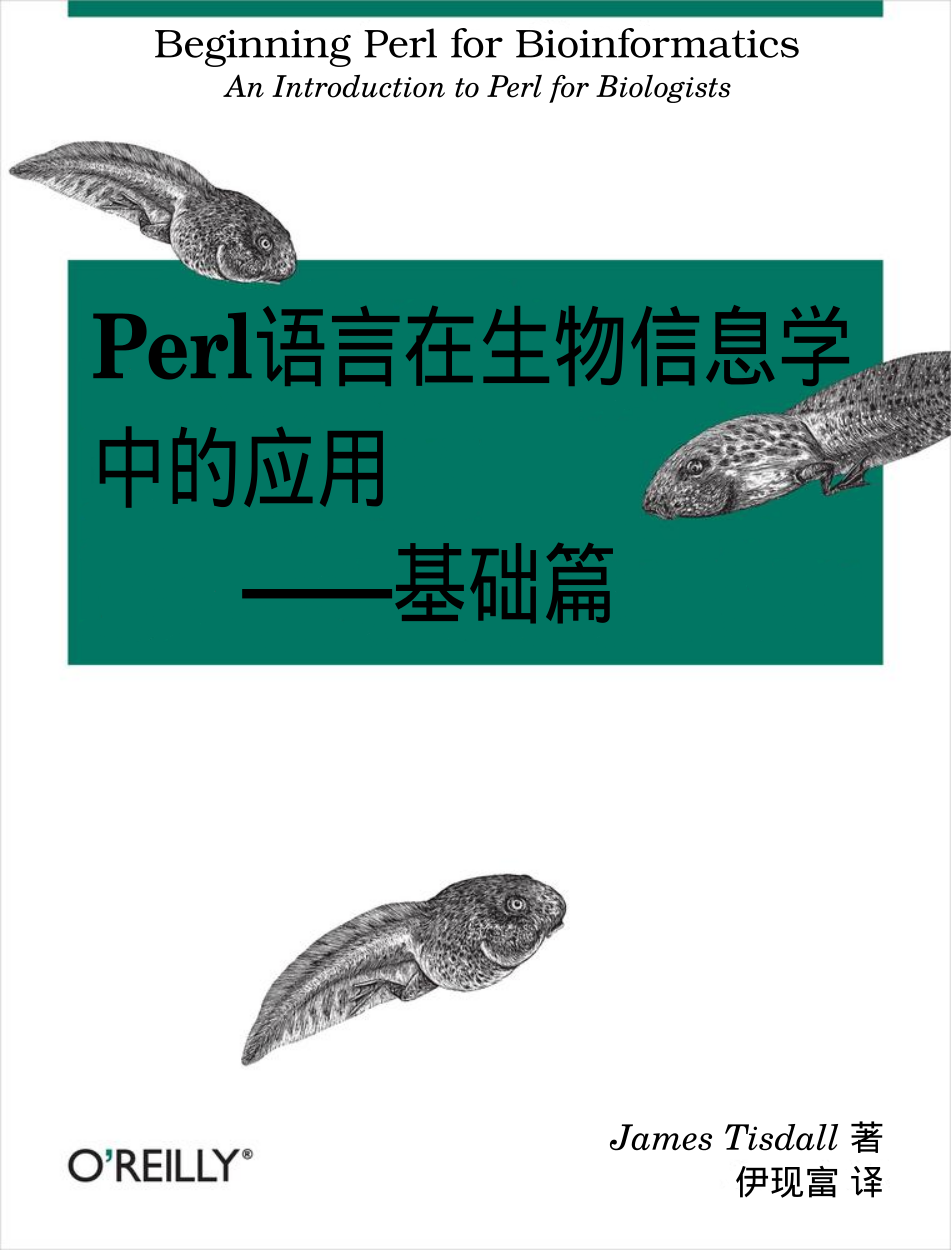
\includegraphics[width=6cm]{c1_intro_textbook.png}
  \end{figure}
\end{frame}

\begin{frame}
  \frametitle{课程安排 | 理论课}
  \begin{center}
  \alert{前9周,每周三/五,\\ 上午后两节(10:00-11:40)/下午前两节(13:30-15:10),\\ 西楼501/510}\\
  \vspace{0.2cm}
  \end{center}
  \begin{block}{授课内容}
    \begin{itemize}
      \item 教材内容:第一章……~第十章
      \item 补充知识:Markdown, Git, ...
    \end{itemize}
  \end{block}
\end{frame}

\begin{frame}
  \frametitle{课程安排 | 理论课 | 自主学习}
  \begin{itemize}
    \item 上课期间以小组形式(建议以宿舍为单位)编写程序
    \item 任务主题不限(兴趣主导,生信方面的最好)
    \item 理论课的最后一/两次课(2~4学时)进行报告
    \item 小组成员人人都要参与
    \item 既参与编程又进行报告者加分
    \item 作为平时成绩的一大部分
  \end{itemize}
\end{frame}

\begin{frame}
  \frametitle{课程安排 | 理论课 | 自主学习 | 实例}
  \begin{block}{目的}
    按照用户的需求生成随机密码。
  \end{block}
  \pause
  \begin{block}{需求}
    \begin{itemize}
      \item 指定生成密码的元素(默认:混合使用数字、大小写字母、符号)
      \item 指定生成密码的长度(默认:12个字符)
      \item 指定生成密码的个数(默认:1个)
      \item 指定密码中元素的比例/字符数(默认:无比例/字符数要求)
      \item 指定需要排除的元素(比如:0和O,1和l;默认:无)
      \item 挖掘更多人性化需求……
    \end{itemize}
  \end{block}
  \pause
  \begin{block}{代码仓库}
    \begin{itemize}
      \item \href{https://github.com/Yixf-Education/project_Perl}{Yixf-Education/project\_Perl}
    \end{itemize}
  \end{block}
\end{frame}

\begin{frame}
  \frametitle{课程安排 | 实验课}
  \begin{center}
  \alert{前9周,每周三,下午前两节(13:30-15:10),教一楼304}\\
  \vspace{0.2cm}
  \end{center}
  \begin{block}{实验内容}
    \begin{itemize}
      \item 紧跟理论课进度
      \item 幻灯片与教材上的程序/实例
    \end{itemize}
  \end{block}
\end{frame}

\begin{frame}
  \frametitle{课程安排 | 考核方式}
  \begin{enumerate}
    \item 理论课:80\%
      \begin{enumerate}
        \item 平时表现:5\%
        \item 课堂测验:5\%(期中)+5\%(期末)
        \item 自主学习:15\%
        \item 闭卷考试:50\%
      \end{enumerate}
    \item 实验课:20\%
      \begin{enumerate}
        \item 平时表现:10\%
        \item 实验报告:10\%
      \end{enumerate}
  \end{enumerate}
\end{frame}

